\documentclass[a4paper,12pt]{article}
\usepackage[top=1in,bottom=1in,left=1in,right=1in]{geometry}
\usepackage[T1]{fontenc}
\usepackage[utf8]{inputenc}
%\usepackage{newunicodechar}
%\usepackage{lmodern}
\usepackage{textgreek}
\usepackage{amsmath}
\usepackage{mathtools}
\usepackage{graphicx}
\usepackage{float}
\usepackage[format=plain,labelfont={bf,it},font=it]{caption}
\usepackage{enumitem}
\usepackage{lipsum}
\usepackage{listings}
\usepackage{pdflscape}
\usepackage{../libraries/pgfgantt}
\usepackage{colortbl}
\usepackage{multirow}
\usepackage{array}


\usepackage{tabularx}
\usepackage{hyperref}
\usepackage{setspace}
\usepackage{subcaption}
\usepackage{tikz}
\usepackage{chngcntr}
\usepackage{longtable}
\usepackage{xcolor,colortbl}
\usepackage{multicol} 
\usepackage{oubraces}
\usepackage{stfloats}

% Bibliography
\usepackage[backend=bibtex,style=numeric,sorting=none]{biblatex}
\addbibresource{references.bib}
\renewcommand*{\bibfont}{\footnotesize}

% Common templates
\usepackage{../templates/templates}

% Figure formatting
\setcounter{tocdepth}{3}
\counterwithin{figure}{subsection}
\counterwithin{table}{subsection}

% Style colours
\definecolor{heading}{HTML}{3298DC}
\definecolor{headingText}{HTML}{FFFFFF} 
\definecolor{darkred}{rgb}{0.6,0,0}


\begin{document}
	\makeTitlePage{Progress Report II}{ELEC0118 Fourth Year MEng Project}
        
	\section{Introduction}
	
	\section{Work Done}
    	\subsection{An Vo}
    	\subsubsection{Progress}

During the previous weeks I have continued to work on on building a system model to simulate data transmission using conventional transmission techniques utilising the same optical channel model used for our autoencoder simulations. The purpose of this model is to provide a comparison between the performance of our autoencoders compared to conventional systems used in the industry.

\begin{itemize}
    \item \textbf{4PAM System Simulation}
    
    I have implemented demodulation techniques to my existing model, firstly by applying a 5th order Bessel filter with cutoff frequency 1/10 of the symbol rate to eliminate high frequency noise due to the optical channel. Pulse shaping is applied before decisions are made for each symbol based on decision levels placed midway between each possible signal level.
    
    \begin{figure}[H]
	\centering
	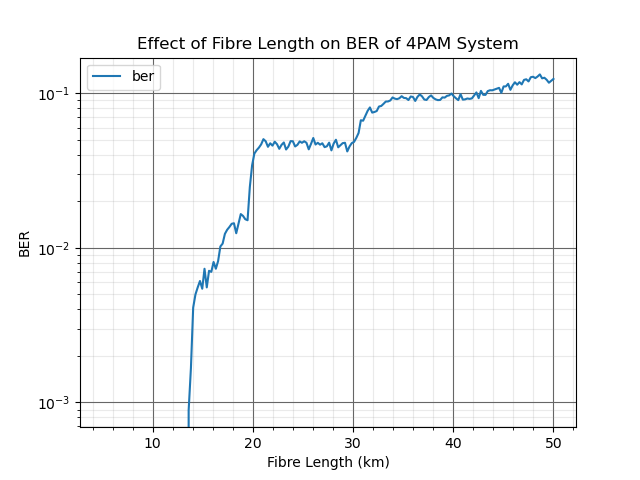
\includegraphics[width=0.9\textwidth]{Fibre Length vs BER.png}
	\caption{Plot of Bit Error Rate of 4PAM system against the fibre length of optical channel}
	\label{fig:output_signal}	
    \end{figure}
    
    By varying the length of the optical channel, the relationship between fibre length and BER can be seen from Figure \ref{fig:output_signal} which will prove to be useful in comparing the performance of the autoencoder system to 4PAM at different cable lengths. The simulation also allows the effects of varying noise and amount of dispersion experienced in the channel to be investigated.
    
    \item \textbf{2PAM System Simulation}
    
    I then changed the system for the 4PAM modulation scheme and reduced it down to provide a 2PAM system that also utilises the same optical channel model used for the autoencoder. 
    
    \item \textbf{OFDM System Simulation}
    
    \begin{figure}[H]
	\centering
	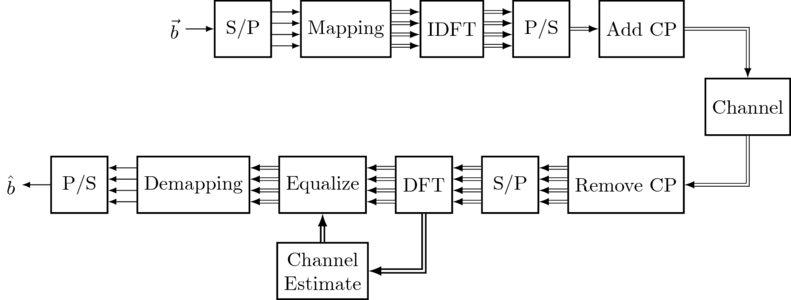
\includegraphics[width=0.9\textwidth]{OFDM diagram.png}
	\caption{Block Diagram containing fundamental blocks for OFDM system}
	\label{fig:OFDM}	
    \end{figure}
    
    The task I am currently working on has been in applying Orthogonal frequency-division multiplexing (OFDM) into a similar system simulation as 2PAM/4PAM which has proved to be more challenging. Time was taken in reading papers and online lectures to understand the concept of OFDM before attempting to apply it in python. I have been implementing each stage of Fig \ref{fig:OFDM} accordingly.
    
    The system utilises 16 QAM modulation scheme and transmits data over 64 subcarriers. Cyclic Prefix is also applied between adjacent OFDM symbols in order to inhibit inter-symbol interference with 25\% of each symbol being the cyclic prefix. Currently I have tested my system on a simple wireless channel that includes an impulse response channel convoluted onto the transmit signal with some additive noise. The next step is to implement the optical channel used in the autoencoder rather than the wireless network and similarly to the 2PAM/4PAM, investigate how the fibre length affects the BER of the system.
\end{itemize}
    	
    	\subsection{Mindaugas Jarmolovi\v{c}ius}
    	
\subsubsection{HDL Neural Network}

A number of modules has been implemented to achieve fully functional neural network:
\begin{itemize}
    \item 32Bit floating point compare unit (greater than, greater equal, less than, less equal)
    \item Cascade adder
    \item Neural module
    \item Layer module
    \item ReLu activation
    \item Hard Sigmoid activation
\end{itemize}

Number of modules have been combined together to test $8 \times 8 \times 2$ network that was trained for 2bit IQ modulation (resulting with modulation that looks similar to 4QAM). Internal neural state was identical to one in simulation, output was slightly different due to hard sigmoid function being used instead of regular sigmoid.


\begin{figure}[H]
    \centering
    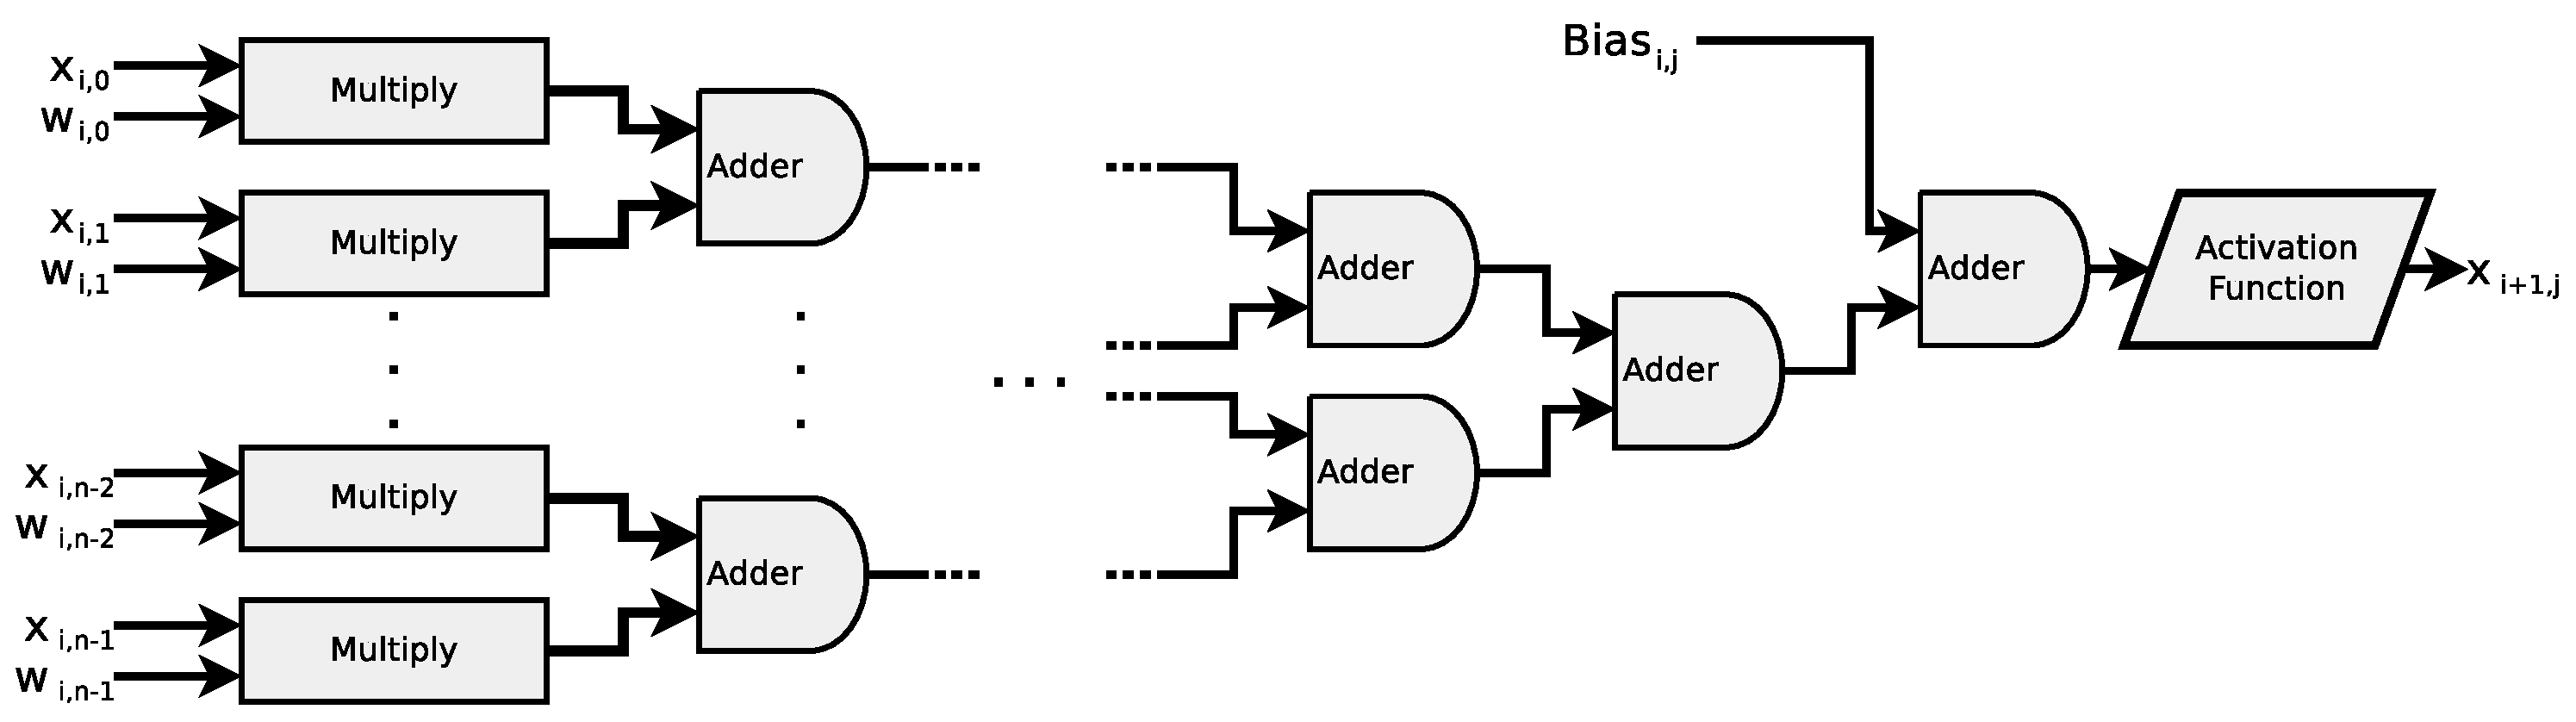
\includegraphics[width=1.05\linewidth]{digital_circ/neuron.eps}
    \caption{Single Digital Neuron Circuit where x is other neuron connection, w - weight, i - layer number, j - neuron number, n - number of neurons in layer.}
    \label{fig:neuron_circ}
\end{figure}

\subsubsection{Cascade Adder}
Cascade adder was the most complex part of the design as module needed to be parameterised. At this point only $2^N$ input signals are considered. Many complications from the fact that this is a dynamically generated module that is not proportional in size - that is 8 input adder would have 3 stages, first having 4 adders, second 2 and last 1. After multiple attempts I concluded that it is impossible to implement this module using conventional loop programming because there is no way set previous and next connections in a single stage as a variable and reuse it in each for loop. Two other solutions were implemented:

\begin{enumerate}
  \item Create a 2D unpacked matrix that contain all connections - this matrix would be $2^{N-1}$ height and $N-1$ width where N is number of stages. Only down side to this solution is that only half of matrix would be always populated because each stage requires twice as many connections. This might not be a problem with a small cascades. HDL synthesizer might optimise such matrix but this needs to be confirmed.
  \item Create a 1D array of connections and calculate indexes of correct connection in each for loop stage. This method required to solve some simple geometric series in order to find index of first connection of each stage at the start of for loop which is shown in \autoref{eq:sum}.
\end{enumerate}

\begin{equation}\label{eq:sum}
    S_n = \sum_{n=0}^m 2^{K-2-n} = 2^{K-2}\frac{2^m-1}{2^m}
\end{equation}
Where K in total number of stages, m is stage.


\subsubsection{Floating Point Arithmetic}

Open source 32 bit floating point arithmetic modules written with SystemVerilog has been adopted to implement neural network. This modules been used for addition and multiplication. It however had three negative sides:
\begin{enumerate}
  \item It uses Synchronous Interconnect Bus shown in \autoref{fig:abus}. When module A is ready to send data, it sends data, sets \textit{stb} (strobe) flat high and freezes until \textit{ack} (acknowledgment) flag is set high by module B indicating that data was accepted. This allows synchronous module communication when each module takes unknown amount of time to compute its input, however downside is that it might wait and idle for input. Also it requires additional signal wires between each module.
  \item Multiplication and addition are implemented as small state machines that move states from taking input, checking for special cases, multiple computing stages and output. Negative side to this is that it takes unknown amount of clock cycles to compute output and it cannot be pipelined, therefore decreasing performance.
  \item These modules are only designed to be used with 32bit floating points, meaning we cannot test lower precision values.
\end{enumerate}

\begin{figure}[H]
    \centering
    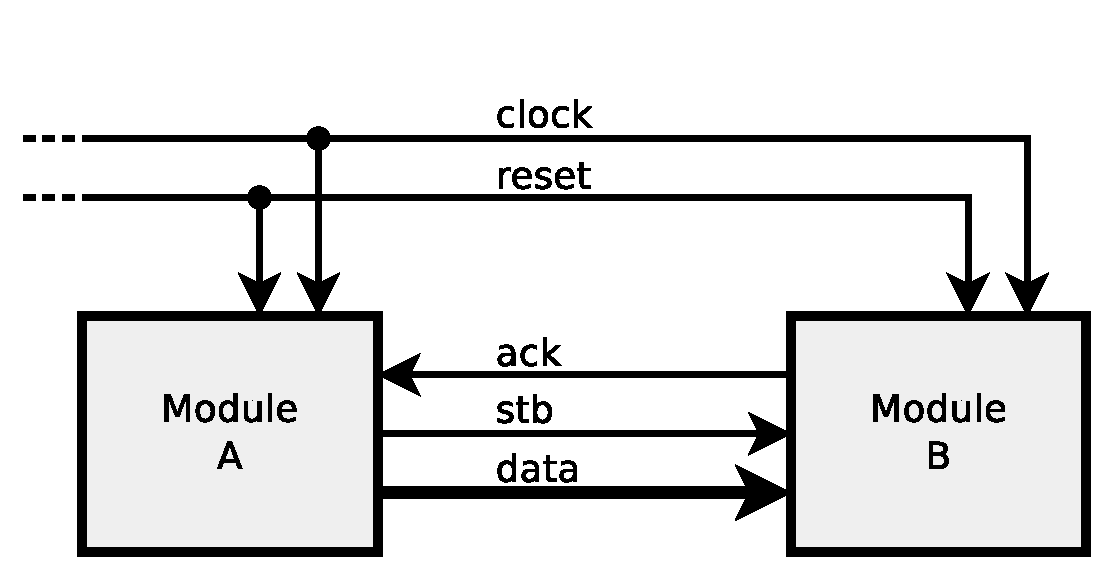
\includegraphics[width=0.4\linewidth]{digital_circ/abus.eps}
    \caption{Synchronous Interconnect Bus Diagram}
    \label{fig:abus}
\end{figure}
        
Due to these reasons, further neural network development in HDL will wait until Oliver finalises better arithmetic operation modules.

    	
    	\subsection{Oliver Jaison}
    	% !TeX root = progress2.tex

\subsubsection{Progress}
Within the last three weeks, my contributions to the project were mainly confined in testing the quality of the signal in the communication channel and the performing product research for future requirements in the project. The details are discussed below. 
\begin{itemize}
    \item \textbf{Create Eye Diagrams}
    
    Upon observing the BERs against certain SNRs of the communication channel it was suggested by Prof. Killey that we implement an Eye Diagram to observe the quality of the transmitted signal to get a better idea of where the error lies. After doing research into some pre-existing Python packages that could perhaps generate an Eye Diagram for us, I decided it was best if I made the function and plots myself. I went through two models of functions to generate an eye diagram before we settled on our current one.
    \begin{figure}[H]
        \begin{subfigure}[h]{0.53\linewidth}
            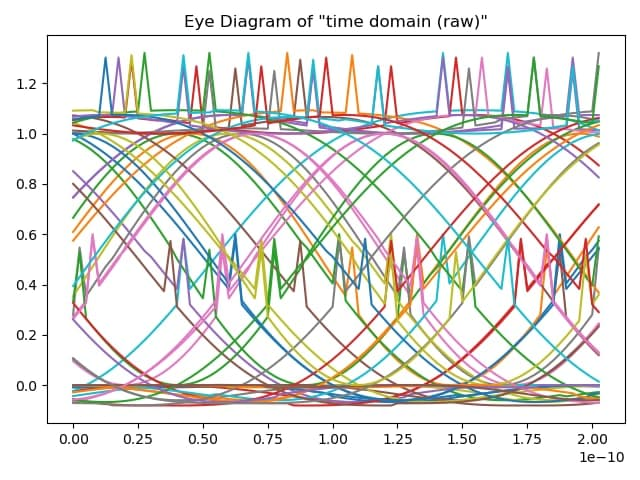
\includegraphics[width=\linewidth]{trial_eye_diagram.jpg}
            \caption{Trial Eye Diagram Model}
        \end{subfigure}
        \begin{subfigure}[h]{0.53\linewidth}
            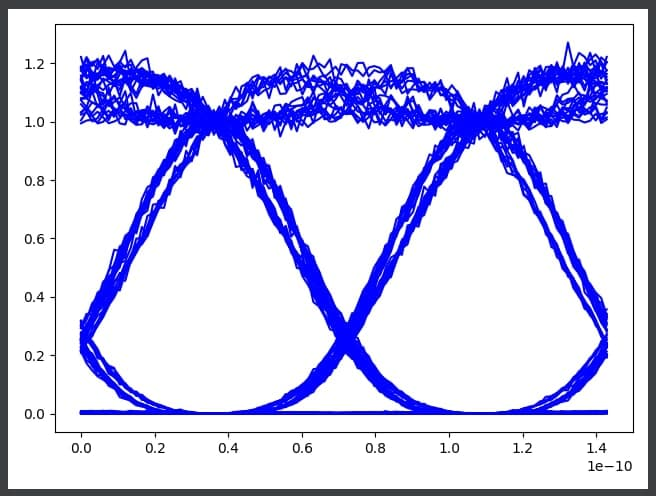
\includegraphics[width=\linewidth]{model_eye_diagram.jpg}
            \caption{Chosen Eye Diagram Model}
        \end{subfigure}
        \caption{Graphs showing the output of the different Eye Diagram Functions}
    \end{figure}
    
    \item \textbf{Research DACs and ADCs}
    
    Currently we are in the simulation stage of our project but after the Christmas holidays we plan to port the model to an FPGA according to our project schedule shown in \textit{\textbf{Table 5.1.1}}. I spent some time researching different DACs and ADCs for the FPGA as suggested by our primary supervisor. After realising that our desired specifications for a DAC/ADC were not feasible (400GSps), I tried lowering the specifications to ~100GSps. This is much more feasible. The majority of my search has been conducted on two companies suggested to me by Prof. Killey: Micram and SocioNext, but I have also looked into Texas Instruments and Fujitsu to see if they have any viable options. At this stage the group are still deciding based on our options. 
\end{itemize}
\subsubsection{Difficulties Encountered}
As I mentioned before, I looked through pre-existing Python packages to see if there was already a function that could build an eye diagram for us and I could just tailor some of the data for that function. As it turned out, none of the packages we had already installed had anything with what I was looking for. I managed to find two packages online but the documentation was scarce and support was little. The results it produces is quite clean and easy to read so I need to spend some time debugging the program. I have not yet been able to do this as we have found another solution that seemed more readily at hand.\newline

In researching product information for DACs and ADCs, I did encounter some difficulty in finding the correct and useful information about the product. I required me to do proper research into our needs and what specifications are generally detailed in each product. Additionally some companies keep this information private and I need to go through UCL as an institution to acquire this product information.
    	
    	\subsection{Tharmetharan Balendran}
    	% !TeX root = progress2.tex

\subsubsection{Progress}

During the last three weeks the key parts of the project that I worked on are the neural network design as well as the optical channel simulation. My individual milestones are discussed below:
\begin{itemize}
    \item \textbf{Finalization of Optical Channel Model}\\
    Having completed the optical channel model in python I was able to simulate BER for different lengths and pulse-shapes for a simple 4-PAM modulation scheme.
    
    \item \textbf{Tweaking Autoencoder Parameters}\\
    I took some time to experiment with different activation functions (leaky/clipped ReLU, softplus, elu and custom activation functions) and regularization techniques such as dropout layers and activation regularizers. Activation regularizers in particular were interesting as they penalize large outputs of a layer and thereby force the output to have a small magnitude. This can be used to penalize the increasing symbol power and prevent the learnt symbols from having extremely large energies to overcome modelled noise. It should be noted that the autoencoder discussed here is a simple prototype and different to that discussed in the next section.
    
    \item \textbf{Replication of Neural Network discussed by B. Karanov et al. \autocite{8433895}}\\
    The neural network configuration discussed in this paper demonstrated promising results and would be a good place to start. An identical implementation of the neural network was configured using tensorflow. To enable this, the optical channel model had to be re-developed to be compatible with tensorflow's tensor datatype. I was able to implement these and learn symbols similar to those discussed in the paper.
    
    \item \textbf{Customization of layers to further decrease BER}\\
    As the chromatic dispersion results in ISI, an encoder/decoder that is able to consider previously received/transmitted symbols should outperform one that solely considers one symbol at a time. To simulate this I started implementing LSTM layers at the encoder and decoder. This is still in progress.
    
\end{itemize}

\subsubsection{Difficulties Encountered}
\begin{itemize}
    \item It is difficult to interpret the exact amount of noise that was simulated in the simulations discussed in \autocite{8433895}. Therefore it is difficult to compare BER achieved by us to those in the paper.
    
    \item With the complexity introduced by the optical channel layer, the autoencoder takes a long time to train on the CPU version of tensorflow. This has been discussed with the project supervisor and access to remote GPU training is being considered.
    
\end{itemize}
	
	\section{Failure Risk Assessment}
	At the moment we are behind of a planned schedule.
	
	\section{Updated Safety Risk Assessment}
    There are no updates on safety risk assessment.
    
    \section{Help and Advice Needed}
    At this state no help is needed, and any small issues are sorted out in weekly supervisor meetings.
	
	
	\newpage
\begin{landscape}
	\subsection{Project Schedule}
	
	\begin{table}[h!]
		\centering
		\begin{ganttchart}[
			y unit title=0.5cm,
			y unit chart=0.5cm,
			x unit=0.92mm,
			hgrid,
			today=2020-12-03,
			today label node/.append style={below=12pt},
			today label font=\itshape\color{blue},
			today rule/.style={draw=blue, ultra thick},
			title height=1,
			bar/.append style={fill=blue!50},
			bar incomplete/.append style={fill=gray!50},
			progress label text={$\displaystyle{#1\%}$},
			time slot format=isodate,
			milestone/.append style={inner sep=2pt, draw},
			title/.style={fill=heading!25, draw=black},
			link/.style={->, ultra thick, style=blue!50!black},
			milestone inline label node/.append style={left=5mm}
			]{2020-10-05}{2021-04-30}
			\gantttitlecalendar{year, month=shortname} \\
			\gantttitle{40}{6}
			\gantttitlelist{41,...,52}{7}
			\gantttitlelist{1,...,16}{7}
			\gantttitle{}{6} \\
			
			\ganttbar[progress=100]{Literature Review}{2020-10-05}{2020-10-22}\\
			\ganttbar[progress=45]{Implementing common NNs}{2020-10-23}{2020-12-06}\\
			\ganttbar[progress=0]{BNN for TensorFlow}{2020-11-29}{2020-12-14}
			\ganttbar[progress=0]{}{2021-01-12}{2021-02-01}\\
			\ganttbar[progress=80]{Channel Model Simulator}{2020-10-23}{2020-11-11}\\
			\ganttbar[progress=0]{Chose and order FPGA}{2020-11-15}{2020-12-14}\\
			\ganttbar[progress=0]{FPGA Tools \& Structures}{2020-11-09}{2020-12-14}
			\ganttbar[progress=0]{}{2021-01-12}{2021-03-14}\\
			\ganttbar[progress=0]{Writing NN on HDL}{2020-11-15}{2020-12-06}
			\ganttbar[progress=0]{}{2021-01-12}{2021-03-21}\\
			\ganttbar[progress=0]{Training COMs model}{2021-02-01}{2021-03-01}\\
			\ganttbar[progress=0]{Porting model to FPGA}{2021-02-25}{2021-03-14}\\
			\ganttbar[progress=0]{Testing model to real COM}{2021-03-14}{2021-04-11}\\
			\ganttbar[progress=0]{Testing FPGA with real COM}{2021-03-21}{2021-04-27}\\
			\ganttbar[progress=0]{Writing final report}{2021-03-27}{2021-04-30}\\
			% 			\ganttlink[link/.append, link type=dr]{elem3}{elem4}
			% 			\ganttlink[link/.append, link type=dr]{elem4}{elem5}
			
			\ganttmilestone{Project Proposal finalised}{2020-10-23}\\			
			\ganttmilestone{Progress Report \#1}{2020-11-11}\\
			\ganttmilestone{Progress Report \#2}{2020-12-02}\\
			\ganttmilestone{December Interim Report}{2020-12-16}\\
			\ganttmilestone{Progress Report \#3}{2021-02-05}\\
			\ganttmilestone{Progress Report \#4}{2021-03-05}\\
			\ganttmilestone{Progress Report \#5}{2021-04-13}\\
			\ganttmilestone{Poster Presentation}{2021-04-17}\\
			\ganttmilestone{Final Report}{2021-04-30}
			\ganttvrule{Reading Week}{2020-11-09}
			\ganttvrule{}{2020-11-15}
			\ganttvrule[vrule label node/.append style={anchor=north west}]{Holidays}{2020-12-18}
			\ganttvrule{}{2021-01-11}
			\ganttvrule{Reading Week}{2021-02-15}
			\ganttvrule{}{2021-02-21}
			\ganttvrule{Term 2 Ends}{2021-03-26}
			\ganttvrule{Term 3 Starts}{2021-04-26}
		\end{ganttchart}	
		\caption{Project schedule and deadlines in a Gantt chart}
		\label{table:time}
	\end{table}
\end{landscape}
	
\end{document}
